\chapter{Tools for the job}
\label{ch:tools}
\doublespacing
\vspace{-2.5cm}

The previous Chapters highlighted the need for a new software architecture that may constitute the foundational layer of distributed autonomous systems, and provided a solid set of requirements that can drive its design. Existing frameworks have been reviewed, some of which provided valuable insights and ideas about how to address some of the design challenges, but none ultimately offering the complete set of features required. Before presenting the design of the solution that this work proposes, it is important to delve further into a point that the previous discussion shed light onto: there are solutions available, in both the literature, the industry, and the open-source software community, that can be employed to address some of the key issues that the requirements identify. Following the computer science design principle recalled in \Cref{sec:prb_requirements}, that is, to not reinvent the wheel, it would be wise to review these tools and see how they can be integrated in the proposed solution. This Chapter provides such an overview: for each tool, its necessity will first be motivated by illustrating a problem that is common in the development of distributed autonomous systems, and then the tool itself will be presented, along with a brief discussion of its features and limitations. Note that the aim of this work is to provide a general-purpose software architecture, so not all of the solutions presented in this Chapter, as well as all the features that the proposed architecture will have, may be necessary or even beneficial in every practical context. However, the goal is to provide a solution that can be adapted to a wide range of applications, as a good toolbox to have at hand, offering a set of features that can be configured and used as needed.

\section{Inter-process communication: the middleware}
\label{sec:middleware}
When developing distributed systems composed of many modules, especially software ones, the transmission of data among them becomes a topic of paramount importance. Note that this issue concerns both transmissions happening between software modules running on the same host and on different hosts. Moreover, alongside this topic there is that of \emph{intra-process communication}, that is, the organization and regulation of data exchanges among different threads running in a same process. Examples of situations in which many software modules may coexist inside a single process, and why such a situation may be desirable, are presented and discussed in the following, for now let us focus on the general problem of inter-process communication and simply note that in the majority of the situations, this other problem can be solved by employing either the same tools that are used for inter-process communication, or simpler ones based on shared memory areas guarded by synchronization primitives.
One has, in general, to figure out a variety of issues such as the following:
\begin{itemize}
  \item \textbf{Data formatting}, \emph{i.e.}, how information that should travel from one module to another should be encoded and structured in packets or similar entities.
  \item \textbf{Data serialization and deserialization}, \emph{i.e.}, how packets should be transformed into a format that can be transmitted over a medium, which is usually some kind of point-to-point connection or a network.
  \item \textbf{Data transmission}, \emph{i.e.}, how packets should be sent and received, and how the system should react to errors or delays in the transmission; this also includes things like reliability requirements, that is, whether the system should guarantee that a packet is delivered, and how many times it should try to deliver it if it fails.
\end{itemize}
The points listed above are usually dealt with by employing a specific \emph{protocol}, that is, a predefined set of rules that regulate all those aspects of the communication. All the software that composes the system should adopt such protocol, which is usually implemented in a set of libraries that can be used in the code. However, dealing directly with networking protocols might slow down the development process: the host system configuration usually becomes very important, since all the operating systems involved must agree on the protocol implementation to support and use, and a lot of work may become necessary to proficiently use all the protocol APIs to achieve all the desired communication features and behaviors. Let us remember that this is not the original task: the goal is to develop a distributed autonomous system, and to write software for it, thus it would be desirable to have a tool that abstracts all the networking details and provides a simple and easy-to-use API that makes data transmission in software modules a straightforward operation, from both the coding and implementation points of view. This is where a particular kind of software, historically denoted by the term \emph{middleware}, comes into play. To grasp its importance in the context of this work, a step back in time is necessary.

In 1968, a conference sponsored by the Science Committee of the North Atlantic Treaty Organization (NATO) was held in Garmisch, Germany, on the topic of software development. Although not widely discussed, it was a historically significant event in this field: it provided a comprehensive overview of the design practices and methodologies used by leading companies in the growing and highly competitive field of computing. The goal was to identify standard strategies for addressing common problems. It should be noted that at that time, and for at least another fifteen years, there were virtually no standards in computer production and programming. Each company offered its own product developed from scratch, in both hardware and software. Standardization and collaboration among various manufacturers began only when information started being exchanged between different computers, first through storage media and later over the Internet, alongside a growing demand for new types of devices and standard formats to adopt when sharing data. A fairly complete transcription of the conference can be found in \cite{naur_software_1969}. It includes the first official mentions of several concepts well known today, such as \emph{component design} and \emph{unit testing}. However, of particular relevance to this work is the representation of the hierarchical structure of software presented by one of the speakers. This structure, valid even today with certain extensions, is illustrated in the inverted pyramid scheme shown in \Cref{fig:swpyramid}.
\begin{figure}[t!]
  \centering
  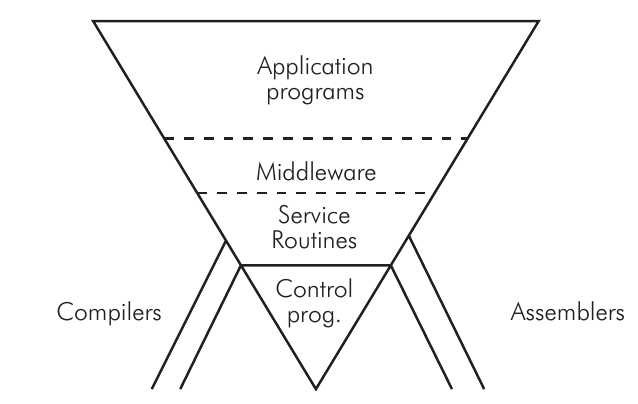
\includegraphics[width=0.8\textwidth]{images/ch3/software_pyramid.png}
  \caption{Software organization in a general-purpose computer, as presented at the 1968 NATO conference on software engineering.}
  \label{fig:swpyramid}
\end{figure}
The idea is that a complex system is like an inverted pyramid: it cannot remain operational without adequate support provided by secondary components. These might be completely invisible to the end user and thus may be considered somewhat external, yet are of vital importance for the correct functioning of the whole: \emph{compilers} and \emph{assemblers}, for instance, which are programs that translate code written in a given language first into the target architecture's assembly language and then into binary machine language, typically generating an executable file at the end of the processing pipeline. These tools must be reliable and efficient, as the implementation of everything else depends on them. Next, we have the layers of \emph{Control Programs} and \emph{Service Routines}: these are what we today call the \emph{operating system} and \emph{device drivers}. They are typically developed with a strong dependence on the machine at hand, considering its specific characteristics, and heavily depend on the employed compilation tools. Their role is to provide an abstraction of the hardware that makes its use simple both for the end user, who interacts with applications, and for application developers themselves. The application software is precisely what we find in the topmost layer: programs that use the hardware more or less directly to provide various services to users. There is, however, an intermediate layer that is often overlooked because it was not always present or was difficult to characterize in the past: the \emph{middleware}. Situated between system software and application software, middleware found its first definition and characterization at the aforementioned conference. Initially conceived merely as a connective layer between current and \emph{legacy} software, middleware provides services and functionalities common to applications beyond what the operating system offers, building itself on top of it and abstracting its own implementation and protocol details. From the perspective offered by the topmost level of the inverted pyramid it appears as normal application software, often consisting of shared or dynamic libraries. Middleware typically offers services to programmers aimed at, \emph{e.g.}, data management, communication, and authentication. Therefore, middleware aids developers in building applications more efficiently by acting as a connective tissue between applications, data, and users. In distributed environments, middleware can facilitate the development and execution of large-scale applications. A typical service offered by middleware is a method for data exchange between applications, even across different devices, according to a common format referred to as an \emph{interface}, which is defined as needed. In general, the services offered by middleware are specified only in terms of their dynamics but can be implemented on different architectures and devices, functioning consistently while keeping their implementation hidden from both the application programmer and the end user. For example, when middleware handles communication between applications, it might position itself within the network stack between the transport and application layers\footnote{Considering the TCP/IP model, which is a four-layers reduction of the original seven-layers Open Systems Interconnection (OSI) model of the networking protocol stack.}. Today, middleware can be categorized into two types: that which operates in \emph{human time}, designed for direct use by human users (\emph{e.g.}, web services), and that which operates in \emph{machine time}, composed mainly of APIs that application developers can use to facilitate their work, benefiting from increased portability across a wide variety of devices. In light of all this, and considering the common difficulties faced when designing the software for a distributed autonomous system, it becomes clear how adopting communication middleware to solve the problem of data exchange among modules can simplify things: many functionalities that would have to be implemented from scratch would instead be offered by the middleware itself as services to be employed in the programs being developed. The selection of this particular class of middleware is again motivated by both the current trends in the software industry pertaining to the development of autonomous systems, and to the author's experience in the field during the years that led to this work.

The rest of this section will introduce three specific middlewares that are widely used in the industry and in the open-source community, and that have become of pivotal importance in the two practical scenarios considered later in this work as a specialization of the proposed architecture: that of autonomous robotics and that of power plants. The first middleware is the \emph{Data Distribution Service} (DDS), which has been the first to provide a standard for data exchange in distributed systems, followed by the Zenoh middleware which addresses some of the limitations of DDS, and finally the \emph{Robot Operating System} (ROS), which is a middleware specifically designed for robotics applications. All these three components will be included in the architecture proposed in the following Chapters, making some of its foundational layers.
